\section*{Contributions}
\addcontentsline{toc}{section}{\protect\numberline{}Main results}

%combining several existing ideas new (\A, trie, seeds)

\dictum{%
   Provably optimal and heuristically fast.}
\vskip 1em

\begin{figure}[h]
  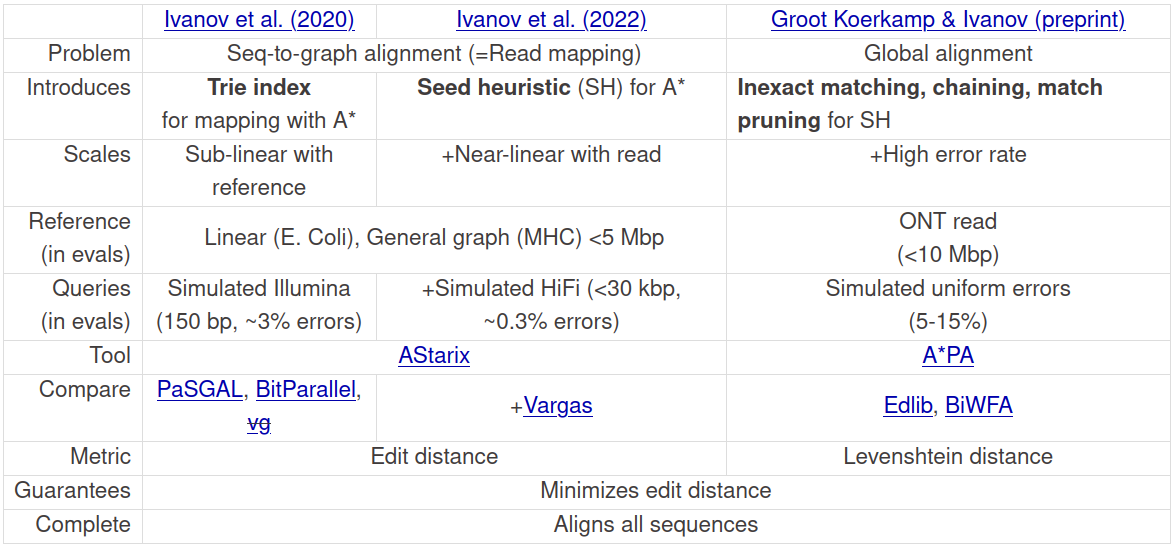
\includegraphics[width=1.0\linewidth]{media/ownpubs-table.png}
  \caption{Overview of the publications.}
  \label{tab:ownpubs}
\end{figure}

In this thesis we consider a novel principled approach that
exploits information from the whole sequences to align sequences provably
optimally and heuristically fast. We empyrically demonstrate the superior
scaling and performance to other optimal alignment algorithms.

We borrow the existing concept of seeds but apply it in a novel way: instead of
finding alignments around seed matches, we use the lack of matches to penalize
alignments by desigining the \emph{seed heuristic} that drive the \A search.
Seeds are cousins of kmers which are popular in sequence alignment since de
Bruijn Graphs were applied for genome assembly. Further kmers are cousins of
ngrams which are popular in computational linguistics since .

We have effectively applied the \A algorithm to optimal sequence alignment. We
demontrated that the additional information from the whole sequence can improve
the scaling with query length, reference size and error rate, substantially
decrease the necessary computations, and result in algorithms that are orders of
magnitude faster than existing optimal algorithms. We apply the \A approach to
two types of alignment: semi-global (alignment) and global.

\subsection*{Principled approach by shortest paths}
shortest paths,

A*, admissibility

\subsection*{Optimality guarantees}
To ensure that our algorithms are practical, we introduce a number of
algorithmic optimizations which increase performance and decrease memory
footprint.

We also prove that all optimizations (greedy matching, ) are preserving the optimality.

\subsection*{Scaling with reference size using a trie index}

%\section{Reconceptualizing seeds for optimal alignment}
\section{Beyond \emph{seed-(chain)-extend}}

As we saw in \cref{ch:trie,ch:seed}, all optimal read mappers compute the whole
dynamic programming table, thus reaching the prohibitively slow quadratic
runtime. On the other side, all current production aligners rely on the
\emph{seed-extend} paradigm (and its \emph{seed-chain-extend} variants for long
reads).

This paradigm requires similar short \emph{seed} patches to be found
between the sequences (\eg by hashed kmers, minimiziers, maximum exact matching,
etc.), and then to \emph{extend} the alignment of the whole query around these
\emph{seeded} similar patches. This is a very intuitiv approach if the goal is
to find a \emph{good alignment}.

If we instead seek not good but provably \emph{best} alignments, we are required
to at least implicitly refute all the exponentially-many competing alignments.

Instead, to find optimal alignments, we do not need to choose the seeds to be
long and similar with the reference buare not required to be similar.

\begin{observation}[Seeds without matches]
    To efficiently find an optimal alignment using \A with the seed heuristic,
    seeds are not required to match (even on the resulting alignment).
\end{observation}

Nevertheless, each seed can penalize potential alignment by not more than its
\emph{potential} (\ie the number of plus $1$, for the case of exact matching
with unit costs). Any additional errors will require more states to be expanded.

This is an interesting observation was made by Ragnar while playing with the
seed heursitic. It looks Indeed, of finding a good alignment but to prove that all
alternative alignments are no better, the seed heuristic for \A search does not
really need matches to be efficient.

This novel usage of seeds carrie different problems and different possibilities.
\section{Analysis of scaling}

% background
Traditionally, the runtime and memory have been analysed for the worst case
asymptotic behavior of the algorithm. Since the near quadratic worst case
asymptotics is likely to be tight for both global~\citep{backurs2015edit} and
semi-global alignment, we targeted related sequences (by limiting their
per-letter error rate), and estimated their empyric runtime and memory scaling.

% issue
The seed heuristic, which is in the core of our \A algorithm, is admissible
(optimistic) but not consistent (monotone). As a consequence, any of the
quadratic number of state can be expanded multiple times, which could
theoretically lead to over-quadratic scaling. In practice, repeated expansions
happen but the empyrical scaling is preserved near-linear as long as the number
of seed matches is near-linear and the seed heuristic is capable of compensating
for the errors.

% empyrical
Our empyrical analysis of scaling is done by repeatedly running the same
algorithm on increasingly more complex input data (\eg longer sequences, higher
error rate). This approach is useful to get a sense of the scaling of the
algorithm and its implementation but it is not asymptotical, includes noise (of
measurements and best-fit estimations), is not trivially applicable to more than
1 dimensions.

% theory
An alternative theoretical analysis would consider the average case (expected)
scaling of our algorithms under a data model. An imaginable result would look
like a connection between the sequence lengths, error rate, and the algorithm
steps (mostly dependant on the number of seed matches and the number of expanded
states). To construct such a connection, a heuristic function will have to be
chosen among a class of seed heuristics (\eg with certain seed length, allowed
number of errors in seed matches, etc.).

% regimes
Our algorithms seem to follow any of the scaling regimes, based on the
capability of the seed heuristic to compensate for all the errors.

% speculations
Based on the empitical evaluations and the intuition behind the algorithms, we
speculate that the sequence length until which our algorithms can scale
near-linearly, can be exponentially increased by lowering the error rate. For
the semi-global alignment, any unit of alignment cost that is not compensated by
the potential of the seed heuristic, leads to a deeper exploration of the trie,
which is grows exponentially until it saturate to quadratic.

\subsection*{Scaling with query length using a seed heuristic}

\subsection*{Scaling with error rate using inexact matching and chaining}

Informed search: Two-stage algorithm, similar to Aho-Corasick, increasingly more information (length, prefix, seeds, chaining seeds, chaining seeds + gaps)

\subsection*{Aligning to general graph references}

\subsection*{Implementations}


\paragraph{Scaling with reference size}
In~\cref{ch:trie} we present the tool \astarix which applies the \A algorithm to
find optimal alignments, based on a domain-specific heuristic and enhanced by
multiple algorithmic optimizations. Importantly, our approach allows for both
cyclic and acyclic graphs including variation and de Bruijn graphs. We
demonstrate that using a trie index we can achieve sublinear scaling of aligning
runtime with reference size, and that \A can scale exponentially better than
\dijkstra with increasing (but small) number of errors in the reads. Moreover,
for short reads, both \astarix and \dijkstra scale better and outperform current
state-of-the-art optimal aligners with increasing genome graph size.
Nevertheless, scaling optimal alignment of long reads on big graphs remained an
open problem.

\paragraph{Scaling with reference size}
In~\cref{ch:seed} we upgrade \astarix with a novel \sh which guides the \A
search by preferring crumbs on nodes that lead towards optimal alignments even
for long reads. This approach enables the scaling of semi-global alignment with
read length.

In~\cref{ch:global} we resolve the third major bottleneck -- handling high error
rates. We presented an algorithm with an implementation in \astarpa solving
pairwise alignment between two sequences. The algorithm is based on \A with a
\sh, inexact matching, match chaining, and match pruning, which we proved to
find an exact solution according to edit distance. For random sequences with up
to $15\%$ uniform errors, the runtime of \astarpa scales near-linearly to very
long sequences ($10^7\bp$) and outperforms other exact aligners. We demonstrate
that on real ONT reads from a human genome, \astarpa is faster than other
aligners on only a limited portion of the reads.

%%%%%%
As it turns out, when the error rate is limited, our optimal solutions
empirically scale near-linearly up to very long sequences. This translates to
many orders of magnitude of runtime speedup compared to state-of-the-art optimal
aligners.
